\input{config.tex} % 导入配置文件
\useSmallCircleItem

%全局字体设置
\UseSongFont     %宋体主题
%UseBlackFont    %黑体主题

\begin{document}

%%%%%%%%%%%%%%%%%%%%%%%%%%%%%%%%%%%%%%%%%%%%%%%%%%%%%%%%%%
%封面页
%%%%%%%%%%%%%%%%%%%%%%%%%%%%%%%%%%%%%%%%%%%%%%%%%%%%%%%%%%
% 1. 定义封面内容
%%%%%%%%%%%%%%%%%%%%%%%%%%%%%%%%%%%%%%%%%%%%%%%%%%%%%%%%%%
\newcommand{\mytitle}{图神经网络入门：\\ 从GNN基础到GCN与RGCN进阶} % \\ 表示强制换行
\newcommand{\myinstitute}{Hebei University of Technology}
\newcommand{\mydate}{June 15, 2025}

% 2. 封面页布局
%%%%%%%%%%%%%%%%%%%%%%%%%%%%%%%%%%%%%%%%%%%%%%%%%%%%%%%%%%
\begin{frame}
  \begin{tikzpicture}[remember picture, overlay]
    % --- 顶部蓝色背景栏 (高度占屏幕的 45%) ---
    \node[fill=midblue, inner sep=0pt, outer sep=0pt, 
          minimum width=\paperwidth, 
          minimum height=0.45\paperheight, 
          anchor=north] at ([yshift=1pt]current page.north) {};
    
    % --- 标题文字 (白色, 加粗, 居中) ---
    % yshift=-0.21\paperheight 确保文字在蓝色栏内垂直居中
    \node[text=white, 
          font=\fontsize{26}{30}\selectfont\bfseries, 
          text width=0.9\paperwidth, 
          align=center] at ([yshift=-0.21\paperheight]current page.north) 
          {\mytitle};
    
    % --- 机构信息 (黑色, 居中) ---
    \node[text=black, 
          font=\Large] at ([yshift=-0.5cm]current page.center) 
          {\myinstitute};
    
    % --- 日期 (黑色, 放在机构下方) ---
    \node[text=black, 
          font=\large] at ([yshift=-1.3cm]current page.center) 
          {\mydate};
          
% --- 校徽 (放在最底部中心，稍微往上提一点) ---
    \node[anchor=center] at ([yshift=-3cm]current page.center) {
        
\includegraphics[height=2.2cm]{image/校徽.png}
    };
  \end{tikzpicture}
\end{frame}

%%%%%%%%%%%%%%%%%%%%%%%%%%%%%%%%%%%%%%%%%%%%%%%%%%%%%%%%%%
%目录页
%%%%%%%%%%%%%%%%%%%%%%%%%%%%%%%%%%%%%%%%%%%%%%%%%%%%%%%%%%
\begin{frame}{Contents}
  \vspace{1em} % 调整间距
  \begin{enumerate}
    \item Introduction
    \item Methodology
    \item Experimental Results
    \item Conclusion
  \end{enumerate}
\end{frame}

%%%%%%%%%%%%%%%%%%%%%%%%%%%%%%%%%%%%%%%%%%%%%%%%%%%%%%%%%%
% 内容页
%%%%%%%%%%%%%%%%%%%%%%%%%%%%%%%%%%%%%%%%%%%%%%%%%%%%%%%%%%
\begin{frame}{Richer convolutional feature}
  \begin{itemize}
    \item APP: Classification (Res2Net-v1b)
      \begin{itemize}
        \item Results on mmdetection
      \end{itemize}
  \end{itemize}
  \vspace{0.5em}
  \centering
  \ThreeLineTable{%
  
    \begin{tabular}{lcccc}
      \toprule
      \textbf{Backbone}      & \textbf{Params} & \textbf{GFLOPs} & \textbf{Top-1 err.} & \textbf{Top-5 err.} \\
      \midrule
      ResNet-101           & 44.6 M  & 7.8  & 22.63 & 6.44 \\
      ResNeXt-101-64x4d    & 83.5 M  & 15.5 & 20.40 & --   \\
      HRNetV2p-W48         & 77.5 M  & 16.1 & 20.70 & 5.50 \\
      Res2Net-v1b-50       & 25.23 M & 4.5  & 19.73 & 4.96 \\
      Res2Net-v1b-101      & 45.2 M  & 8.3  & 18.77 & 4.64 \\
      \bottomrule
    \end{tabular}
    
  }
\end{frame}

%%%%%%%%%%%%%%%%%%%%%%%%%%%%%%%%%%%%%%%%%%%%%%%%%%%%%%%%%%
% 项目列表页
%%%%%%%%%%%%%%%%%%%%%%%%%%%%%%%%%%%%%%%%%%%%%%%%%%%%%%%%%%
\begin{frame}{\textcolor{midblue}{D}\textcolor{myred}{O}\textcolor{mygreen}{C}\textcolor{mypurple}{X} 行动倡议}
  \begin{columns}
    \column{0.5\textwidth}
    \begin{itemize}
      \item \textcolor{midblue}{D}emo: 方便科普和教学
      \item \textcolor{myred}{O}pen source: 方便同行复现与验证
      \item \textcolor{mygreen}{C}hinese: 提供中文版论文
      \item e\textcolor{mypurple}{X}plain: 及时回应项目主页上读者提问
    \end{itemize}
    \column{0.5\textwidth}
    \begin{figure}
      \centering
      \includegraphics[width=0.5\textwidth]{image/image1.png}
      \caption{示例图片}
    \end{figure}
  \end{columns}
\end{frame}

%%%%%%%%%%%%%%%%%%%%%%%%%%%%%%%%%%%%%%%%%%%%%%%%%%%%%%%%%%
% 两栏内容示例页
%%%%%%%%%%%%%%%%%%%%%%%%%%%%%%%%%%%%%%%%%%%%%%%%%%%%%%%%%%
\begin{frame}{Two-Column Example}
\begin{columns}
    \column{0.5\textwidth}
    \begin{itemize}
        \item \textbf{Left Column Content}
        \begin{itemize}
            \item Item 1
            \item Item 2
            \item Item 3
        \end{itemize}
        \item \textbf{More Content}
        \begin{itemize}
            \item Subitem 1
            \item Subitem 2
        \end{itemize}
    \end{itemize}
    
    \column{0.5\textwidth}
    \begin{itemize}
        \item \textbf{Right Column Content}
        \begin{itemize}
            \item Item A
            \item Item B
            \item Item C
        \end{itemize}
        \item \textbf{Additional Content}
        \begin{itemize}
            \item Subitem X
            \item Subitem Y
        \end{itemize}
    \end{itemize}
\end{columns}
\end{frame}

%%%%%%%%%%%%%%%%%%%%%%%%%%%%%%%%%%%%%%%%%%%%%%%%%%%%%%%%%%
% 图像页
%%%%%%%%%%%%%%%%%%%%%%%%%%%%%%%%%%%%%%%%%%%%%%%%%%%%%%%%%%
\begin{frame}{Image}
  \begin{itemize}
    \item The example image is as follows
  \end{itemize}
  \begin{figure}
    \centering
    \includegraphics[width=0.68\textwidth]{image/demo.jpg}
    \caption{示例图片\cornerfootnote{仅用于示范}}
  \end{figure}
\end{frame}

%%%%%%%%%%%%%%%%%%%%%%%%%%%%%%%%%%%%%%%%%%%%%%%%%%%%%%%%%%
% 插入公式推导页
%%%%%%%%%%%%%%%%%%%%%%%%%%%%%%%%%%%%%%%%%%%%%%%%%%%%%%%%%%
\begin{frame}{Annual Performance Metrics}
  Key Equation Analysis

  \vspace{1em}

  \begin{center}
    \BehindEqBox{
      $\displaystyle
      S = \underbrace{\sum_{i=1}^{N} \textcolor{myorange}{w_i}\, \textcolor{mygreen}{s_i}}_{\textcolor{midblue}{\textbf{Core Score}}} \;+\;
      \overbrace{\left( {\frac{1}{N} \sum_{j=1}^{M} \textcolor{myred}{\delta_j}} \right)}^{\textcolor{mypurple}{\textbf{Adjustment Factor}}}
      $
    }
  \end{center}

  \vspace{1em}

  % 解释公式变量
  \[
    \left\{
    \begin{aligned}
      \textcolor{mygreen}{s_i} &\;=\; \text{Standardized score for module } i, \\
      \textcolor{myorange}{w_i} &\;=\; \text{Weight assigned to module } i, \\
      \textcolor{myred}{\delta_j} &\;=\; \text{External adjustment from factor } j.
    \end{aligned}
    \right.
  \]

  \vspace{1em}

  \textbf{Remark:} Here, \(S\) represents the overall performance metric of an annual study. The \textcolor{midblue}{Core Score} is the weighted sum of standardized scores \(s_i\), while the \textcolor{mypurple}{Adjustment Factor} accounts for external influences aggregated via \(\delta_j\).

\end{frame}


% 另一种配置说明 %%%%%%%%%%%%%%%%%%%%%%%%%%%%%%%%%%%%%%%%%%%%%

\begin{frame}{Modified Example}
  \textbf{Usage Example:} Configuration: Background color = \texttt{mypurple}, border=1pt, dashed border.
  \vspace{1em}

%dotted

  \begin{center}
    \BehindEqBox[color=mypurple, style=dashed, border=1pt]{$\displaystyle \int_{0}^{1} x^2\,dx = \frac{1}{3}$}
  \end{center}

  \vspace{1em}

  % 其他公式或内容
  \textbf{Remark:} The formula calculates the definite integral of \(x^2\) over the interval \([0,1]\), representing the area under the curve.
\end{frame}

%%%%%%%%%%%%%%%%%%%%%%%%%%%%%%%%%%%%%%%%%%%%%%%%%%%%%%%%%%
%文字强调块
%%%%%%%%%%%%%%%%%%%%%%%%%%%%%%%%%%%%%%%%%%%%%%%%%%%%%%%%%%
\begin{frame}{Types of Text Emphasis}
In this slide, key concepts will be \alert{emphasized} because they are crucial.  
Please use sparingly to maintain clarity.

\vspace{0.5em}
\begin{block}{Information Block}
This is a general informational block.
\end{block}

\vspace{0.5em}
\begin{alertblock}{Warning}
This is important information inside a red alert block.
\end{alertblock}

\vspace{0.5em}
\begin{exampleblock}{Key Takeaways}
This block highlights essential information in a green box.  
The title of the block is "Key Takeaways".  
Here's an additional line for checking vertical spacing consistency.
\end{exampleblock}

\end{frame}

%%%%%%%%%%%%%%%%%%%%%%%%%%%%%%%%%%%%%%%%%%%%%%%%%%%%%%%%%%
%图表
%%%%%%%%%%%%%%%%%%%%%%%%%%%%%%%%%%%%%%%%%%%%%%%%%%%%%%%%%%
\begin{frame}{Bar charts}

\begin{center}
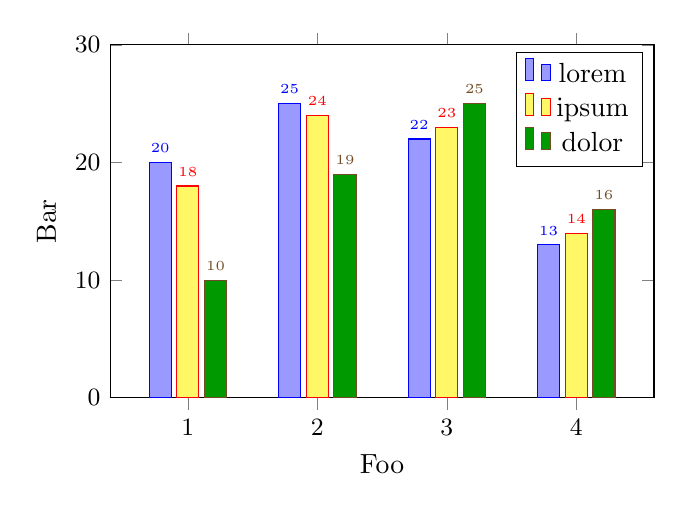
\begin{tikzpicture}
\begin{axis}[
    ybar,
    bar width=8pt,
    width=0.7\textwidth,
    height=0.5\textwidth,
    enlarge x limits=0.2,
    ylabel={Bar},
    xlabel={Foo},
    symbolic x coords={1,2,3,4},
    xtick=data,
    ymin=0,
    ymax=30,
    legend style={at={(0.98,0.98)}, anchor=north east},
    nodes near coords,
    nodes near coords align={vertical},
    every node near coord/.append style={font=\tiny},
    tick label style={font=\small},
]
\addplot+[style={fill=blue!40}] coordinates {(1,20) (2,25) (3,22) (4,13)};
\addplot+[style={fill=yellow!60!white}] coordinates {(1,18) (2,24) (3,23) (4,14)};
\addplot+[style={fill=green!60!black}] coordinates {(1,10) (2,19) (3,25) (4,16)};
\legend{lorem, ipsum, dolor}
\end{axis}
\end{tikzpicture}
\end{center}

\end{frame}

% 问答页
\begin{frame}{Questions and Answers}
  \centering
  \vspace{0.8cm}
  {\Huge \bfseries Q\&A}
\end{frame}

%结束页
\begin{frame}[plain]
  \begin{tikzpicture}[remember picture,overlay]
    % 背景设置：使用深蓝色半透明背景
    \node[fill=midblue, opacity=1, minimum width=\paperwidth, minimum height=\paperheight] at (current page.center) {};
    % THANKS 文本设置：白色大字号
    \node[font=\fontsize{40}{70}\selectfont\bfseries, text=white] at (current page.center) {THANKS};
  \end{tikzpicture}
\end{frame}

\end{document}
